\chapter{Metodologia}\label{ch:work}
\section{JPEG AI Verification Model}\label{sec:vm}
%tipi dei dati, struttura, target bpp e altri parametri.
Lo strumento utilizzato per ottenere la codifica JPEG AI è "jpeg-ai-reference-software" \cite{jpeg-ai-ref-sw} che rappresenta il software di riferimento per la prima implementazione del sistema proposto chiamato \textit{JPEG AI Verification Model} \cite{wg1n100279}. Sono proposti due encoder con diversi livelli di complessità: \texttt{Enc0}, il più semplice, progettato per dispositivi mobili, ed \texttt{Enc1}, più complesso, composto da \textit{attention blocks} e\textit{ transformer}, necessitando quindi capacità computazionale elevata.
Sono supportati tre diversi "operation point" SOP (\textit{Simple Operation Point}), BOP (\textit{Basic Operation Point}) e HOP (\textit{High Operation Point}) ottimizzati rispettivamente per l'uso su dispositivi dotati di CPU, dispositivi mobili, e dispositivi dotati di hardware specializzato come le GPU.
\begin{figure}
    \centering
    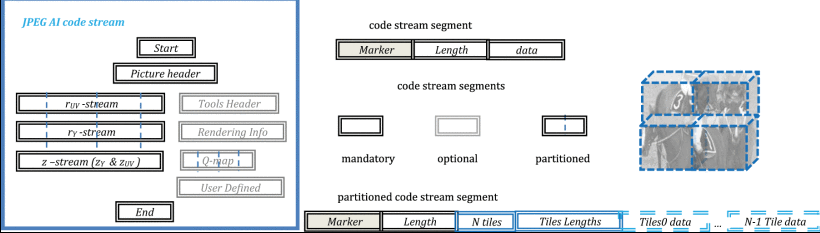
\includegraphics[width=1\linewidth]{img/JPEG AI codestream.png}
    \caption{JPEG AI bitstream}
    \label{fig:bitstream}
\end{figure}
% PARLARE DI VARIABILE RATE O BRM?
\section{Dataset utilizzato}\label{sec:dataset}
Il dataset usato negli esperimenti è \textit{140k Real and Fake Faces} \cite{140kRealFake}, una raccolta di 140.000 immagini di volti, suddivise in 70.000  immagini reali e 70.000 immagini fake.
I dati sono già suddivisi in training set, test set, e validation set, rispettivamente composti da 100.000, 20.000 e 20.000 immagini; ogni insieme mantiene un perfetto bilanciamento tra le due classi; queste caratteristiche rendono il dataset ideale per l'addestramento semplificando la preprarazione dei dati. Le immagini sono in formato JPEG e sono state ridimensionate in 256x256 pixel; sono inclusi file csv contententi le etichette e il percorso di ogni immagine.
\paragraph{Immagini reali}Le immagini reali fanno parte del dataset \textit{Flickr-Faces-HQ} (FFHQ) \cite{NVlabsFfhqdataset2025}, il dataset creato per lo sviluppo di StyleGAN, e consistono in fotografie di volti umani di alta qualità (risoluzione a 1024x1024). Questo si distingue da altri dataset per la presenza di una grande varietà di soggetti per età ed etnia, ma anche per la presenza di accessori come occhiali o cappelli \cite{karras2019style} rendendolo molto diversificato; queste immagini sono state collezionate da Flickr, un servizio web che offre la possibilità di pubblicare immagini ad artisti e fotografi.
\paragraph{Immagini sintetiche}Le immagini fake invece fanno parte del dataset \textit{1 Milion Fake Faces} ,un insieme di immagini generate tramite StyleGAN (vedi sez. \ref{par:style}). 
\section{Classificatori utilizzati}
Sono stati scelti due diversi algoritmi di classificazione, Random Forest e GradientBoosting, entrambi appartenenti alla categoria degli \textit{ensemble methods}. Questi si basano sull'idea di combinare le predizioni di più modelli base detti 'deboli' (\textit{weak learners}) per creare un modello finale con maggior accuratezza e riducendo distorsione e varianza rispetto all'uso di un singolo modello.
\subsection{Random Forest}
Random Forest è un algoritmo di apprendimento supervisionato che utilizza alberi di decisione come modelli deboli.
\paragraph{Alberi di decisione}
Gli alberi di decisione sono algoritmi di apprendimento automatico che rappresentano funzioni che mappano dati in input su un insieme di classi (per problemi di classificazione) attraverso una serie di test rappresentabili con strutture ad alberi. Una volta costruito l'albero di decisioni, la classificazione di un nuovo dato consiste semplicemente nel partire dalla radice e valutare l'esito di ogni test che si incontra. La costruzione si basa sul concetto di ripartizione ricorsiva dello spazio di input in sottinsiemi più piccoli in base ai valori degli attributi. La scelta dell'attributo da usare per la ripartizione viene fatta valutando il guadagno informativo derivato da quella scelta, cercando di minimizzare l'impurità dei sottoinsiemi.
%Misure di purezza
L'aspetto critico di questa tecnica è l'alta varianza, infatti cambiamenti nei dati di addestramento influenzano molto la struttura dell'albero finale.
\paragraph{Random Forest}
I Random Forest \cite{breiman2001random} risolvono questo problema  combinando la tecnica di \textit{bagging} con la selezione casuale di attributi.
Il bagging (Bootstrap Aggregating) consiste nel creare $K$ diversi sottoinsiemi campionando con reinserimento (\textit{Bootstrap}) dall'insieme di addestramento originale. Su ogni sottoinsieme verrà addestrato un modello base, e la predizione finale viene fatta aggregando (\textit{Aggregating}) le predizioni dei $K$ modelli; per i problemi di classificazione si può usare la media o il voto di maggioranza
\begin{equation}
    y = \frac{1}{k}\sum_{i=1}^{k} y_i
\end{equation}
dove $y_i$ è la predizione del modello $i$. Il bagging permette una riduzione della varianza, ma presenta un problema riguardante la forte correlazione che i modelli base tendono ad avere, sopratutto quando un attributo risulta avere un guadagno informativo più alto, diventando radice per molti alberi.\\
Nei Random Forest questo problema viene risolto variando in ogni nodo l'insieme di attributi tra cui poter scegliere quello su cui poi fare il test, garantendo una bassa correlazione tra gli alberi.
\subsection{Gradient Boosting}
Il Gradient Boosting è un algoritmo di apprendimento supervisionato molto popolare per problemi nei quali i dati sono tabellari. La differenza principale rispetto ai random forest risiede nell'uso del \textit{boosting}.
Il boosting introduce l'idea insieme di addestramento pesato, dove ogni esempio ha un peso che indica la sua importanza nell'addestramento. L'idea è quella di allenare un insieme di modelli deboli in modo sequenziale: inizialmente ad ogni esempio viene assegnato lo stesso peso, e su questo insieme viene addestrato il primo modello. Prima di allenare il modello successivo, i pesi degli esempi vengono aggiornati facendo sì che il peso degli esempi classificati in modo errato venga incrementato, mentre quello degli esempi classificati correttamente viene ridotto. Iterando il processo per $K$ iterazioni vengono prodotti $K$ modelli deboli tra i quali almeno un modello riuscirà a classificare in modo corretto anche gli esempi più difficili.\\
Per fare la predizione, ogni modello debole vota, e la predizione finale viene fatta considerando il voto di maggioranza.\\
Nel Gradient Boosting, il processo di boosting non si basa sui pesi, ma sul gradiente negativo della funzione di perdita: si parte con una funzione di perdita differenziabile, si fanno le predizioni e si calcola per ogni esempio il gradiente negativo della funzione di perdita. Con questa informazione viene addestrato un nuovo modello debole aggiornando i parametri muovendosi nella direzione del gradiente negativo. 
\subsection{Hyperparameter Tuning}\label{subsec:tuning}
Le prestazioni dei modelli di apprendimento spesso dipendono dalla scelta degli iperparametri, parametri che riguardano l'architettura/classe dei modelli. Questi non vengono appresi automaticamente, ma anzi sono considerabili come variabili di configurazione da specificare prima di procedere con l'addestramento. Per questo è buona pratica adottare la tecnica di \textit{hyperparameter tuning} per trovare la combinazione di iperparametri che offre migliori prestazioni, che verrano poi utilizzate per creare il modello finale da allenare.
La ricerca viene fatta scegliendo modello e lo spazio dei valori degli iperparametri da esplorare. Negli esperimenti sono state usate la ricerca a griglia (\textit{GridSearch}) e la ricerca casuale (\textit{Random Search}).\\
La ricerca a griglia compie una ricerca esaustiva sulla griglia degli iperparametri specificati, generando un modello per ogni combinazione possibile. Questa, anche se molto onerosa dal punto di vista computazionale, garantisce di trovare la combinazione ottimale tra quelle specificate.\\
La ricerca casuale invece effettua un campionamento di un numero finito di parametri seguendo una distribuzione scelta. Questa tecnica risulta molto meno dispendiosa rispetto alla ricerca a griglia, riuscendo comunque a trovare buone combinazioni di iperparametri; viene usata principalmente quando lo spazio di ricerca ha alta dimensionalità.\\
Per la valutazione dei modelli viene utilizzata la \textit{k-fold cross-validation}, un'operazione che suddivide l'insieme di addestramento in $k$ sottoinsiemi, e addestra il modello su k-1 sottoinsiemi per poi testarlo su quello rimanente; il modello scelto sarà quello che ha ottenuto una migliore accuratezza.
\section{Addestramento dei classificatori}
\subsection{Rappresentazioni latenti estratte da JPEG AI}\label{subsec:latenti}
Le immagini prima di essere elaborate dall'encoder vengono preprocessate: inizialmente sono convertite nello spazio di colori YUV BT.709, separando le componenti di luminanza e crominanza. Successivamente viene applicato la CCS (\textit{Conditional Color Separation}) \cite{10018070}, un approccio per cui la componente primaria, la luminanza ($Y$), viene compressa con una rete neurale più potente, mentre per le componenti di crominanza ($UV$) la compressione avviene sfruttando informazioni della luminanza.
La separazione delle componenti è mantenuta anche nel bitstream finale (vedi fig. \ref{fig:bitstream}) dando la possibilità di scartare la parte di crominanza se non necessaria per l'applicazione scelta.\\
L'encoder genera un dizionario che raccoglie tutti i valori necessari utilizzati nel resto dell'architettura (vedi fig. \ref{fig:architmin}), ma quelli di nostro interesse sono $y$ ed $\hat{y}$, entrambi composti da tensori \texttt{model-y} e \texttt{model-uv} per rappresentare componenti di luminanza e crominanza separatamente come voluto da meccanismo di CCS. Questi tensori hanno rispettivamente dimensione (160, 16,16) per la luminanza e (96, 16, 16) per la crominanza.\\
$y$ rappresenta l'output dell'\textit{Analysis transform} (vedi fig.\ref{fig:encodingJPEGAI}) mentre $\hat{y}$ rappresenta l'input dell'\textit{Synthesis transform} (vedi fig. \ref{fig:decodingJPEGAI}).
\subsection{Preprocessing dei latenti}\label{sec:preprocessing}
Per allenare i modelli di classificazione scelti è necessario trasformare i tensori prodotti dall'encoder in vettori unidimensionali; si sono state utilizzate diverse strategie.
\paragraph{Flattening} La prima strategia testata è stata quella più semplice ed intuitiva da realizzare, trattandosi di una semplice operazione di \textit{flattening} del tensore: dopo aver concatenato le componenti di luminanza e crominanza, ottenendo un tensore di dimensione $(256, 16, 16)$, viene trasformato in un vettore di contenente $65536$ valori.
\paragraph{Estrazione di patch} La seconda strategia adottata consiste nell'estrazione di patch dalle rappresentazioni latenti, dove ogni patch è la concatenazione dei valori presenti in una posizione spaziale (x,y) per tutti i canali (di dimensione 16x16) del tensore. In questo modo si ottiene un vettore di dimensione inferiore rispetto all'uso della tecnica di flattening. Questo approccio permette di aumentare il numero di campioni disponibili per l'addestramento, e renderà l'addestramento più rapido.
